\section{Experiments and results}\label{sec:chp6:exp-res}
To evaluate different aspects of the proposed \ac{cad} system, we proposed variety of experiments with respect to individual modalities and their combination. 
Table~\ref{tab:exp-summary} represents the summary of the experiments. 
These experiments and the results obtained are discussed in details in the reminder of this section. 

\subsection{Experiment-1:}\label{subec:chp6:exp-res:Ex1} 

\begin{figure}
  \hspace*{\fill}
  \subfigure[]{\label{fig:}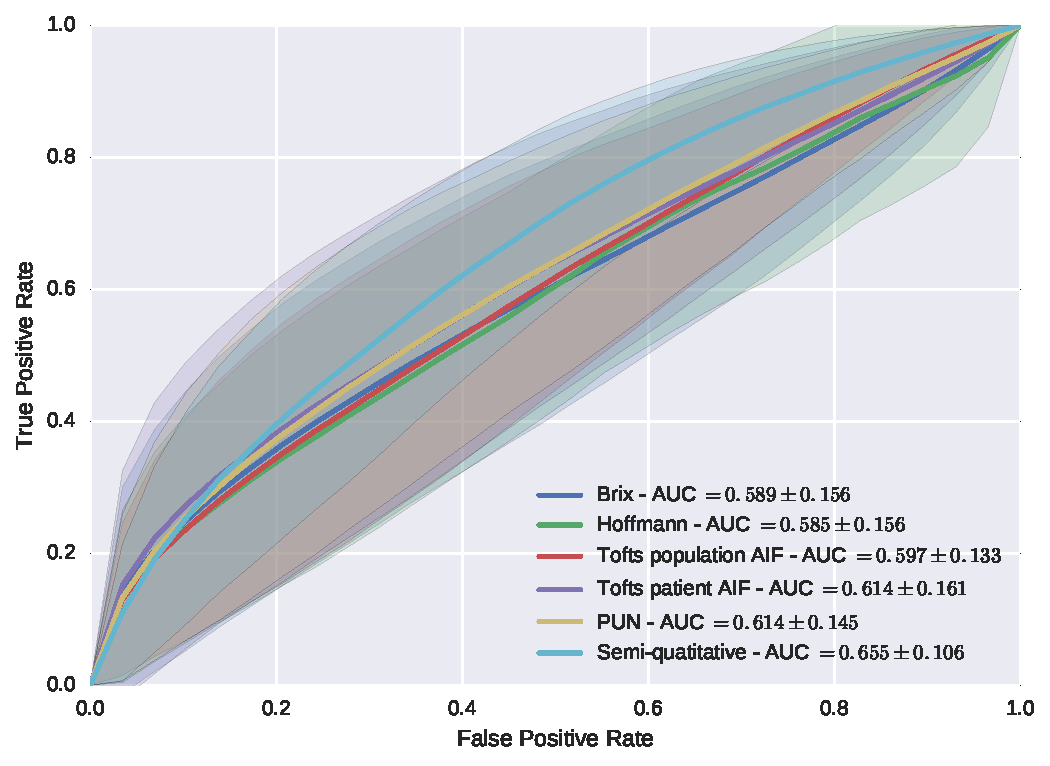
\includegraphics[width=.49\textwidth]{5_normalization/figures/DCE-normalization/normalized_methods_0.pdf}}
  \hfill
  \subfigure[]{\label{fig:}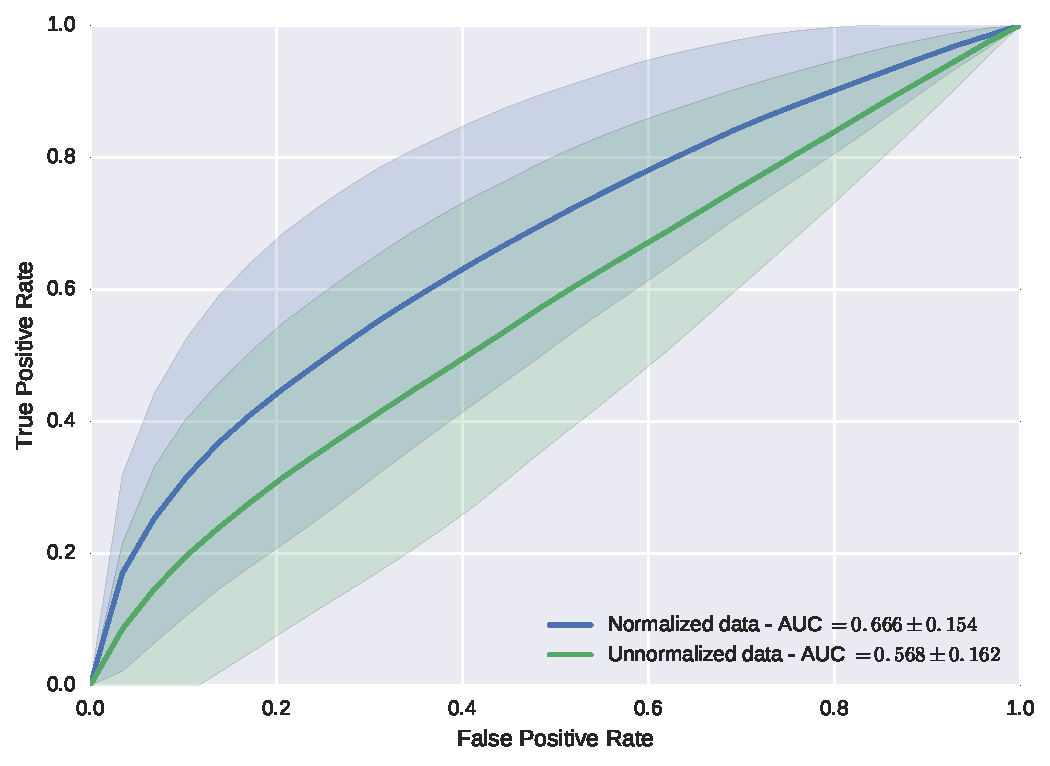
\includegraphics[width=.49\textwidth]{5_normalization/figures/DCE-normalization/full_signal_0.pdf}}
  \hspace*{\fill} \\
  \hspace*{\fill}
  \subfigure[]{\label{fig:}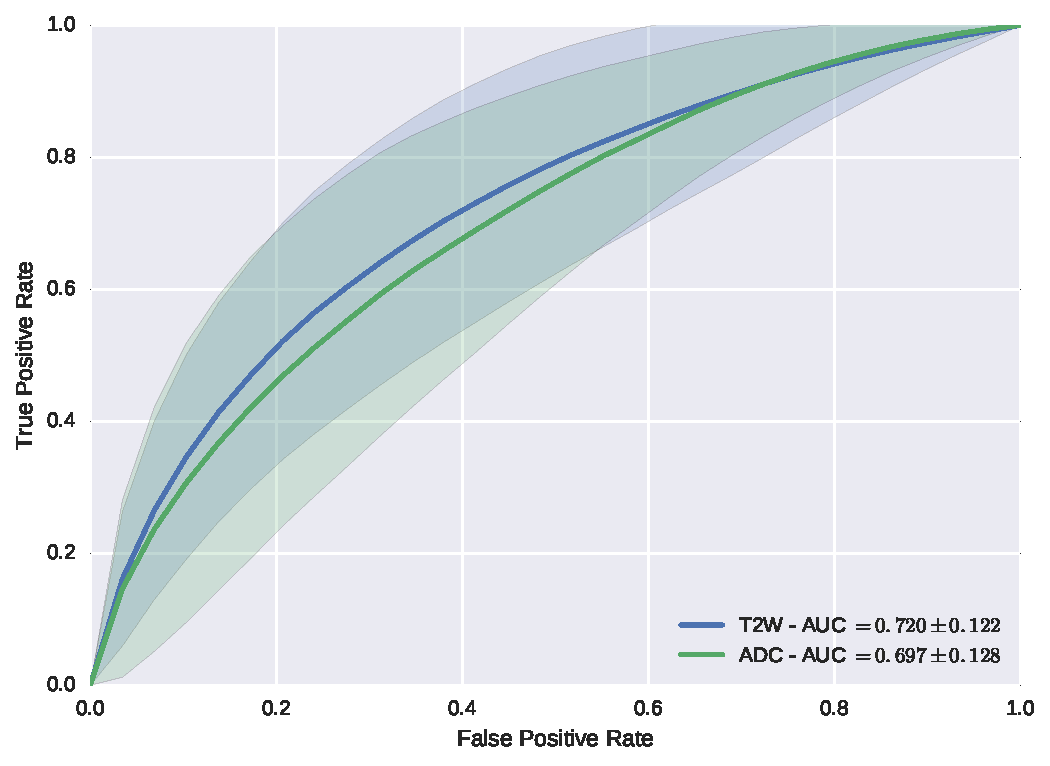
\includegraphics[width=.49\textwidth]{6_pipeline/figures/exp-1/t2w_adc.pdf}}
  \hfill
  \subfigure[]{\label{fig:}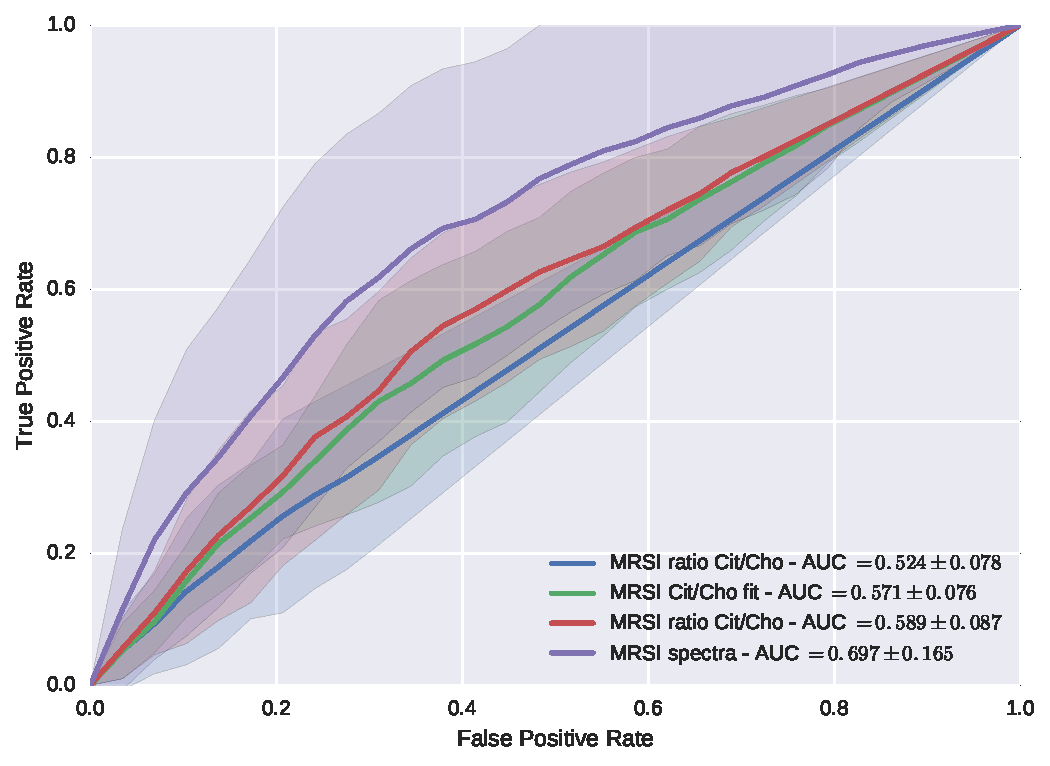
\includegraphics[width=.49\textwidth]{6_pipeline/figures/exp-1/mrsi_all.pdf}}
  \hspace*{\fill}
  \caption{Experiment 1:}
  \label{fig:}
\end{figure}

\begin{figure}
  \centering
  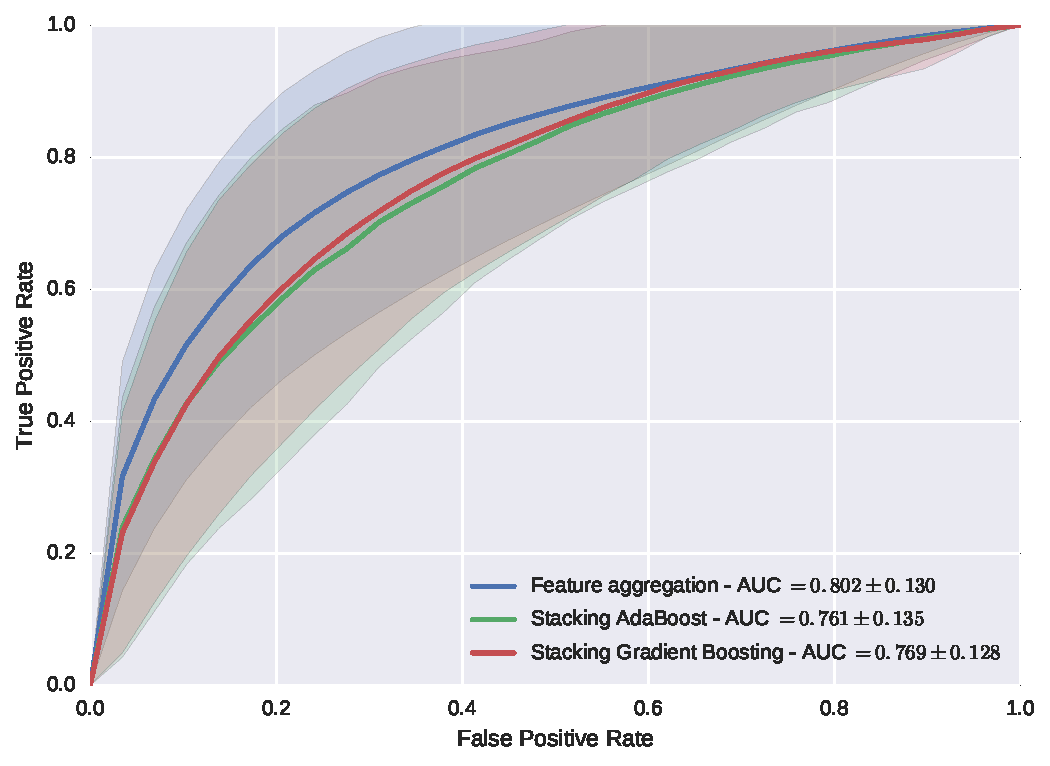
\includegraphics[width=0.7\linewidth]{6_pipeline/figures/exp-2/comb_all.pdf}
  \caption{Experiment 2:}
  \label{fig:}
\end{figure}

\begin{figure}
  \hspace*{\fill}
  \subfigure[]{\label{fig:}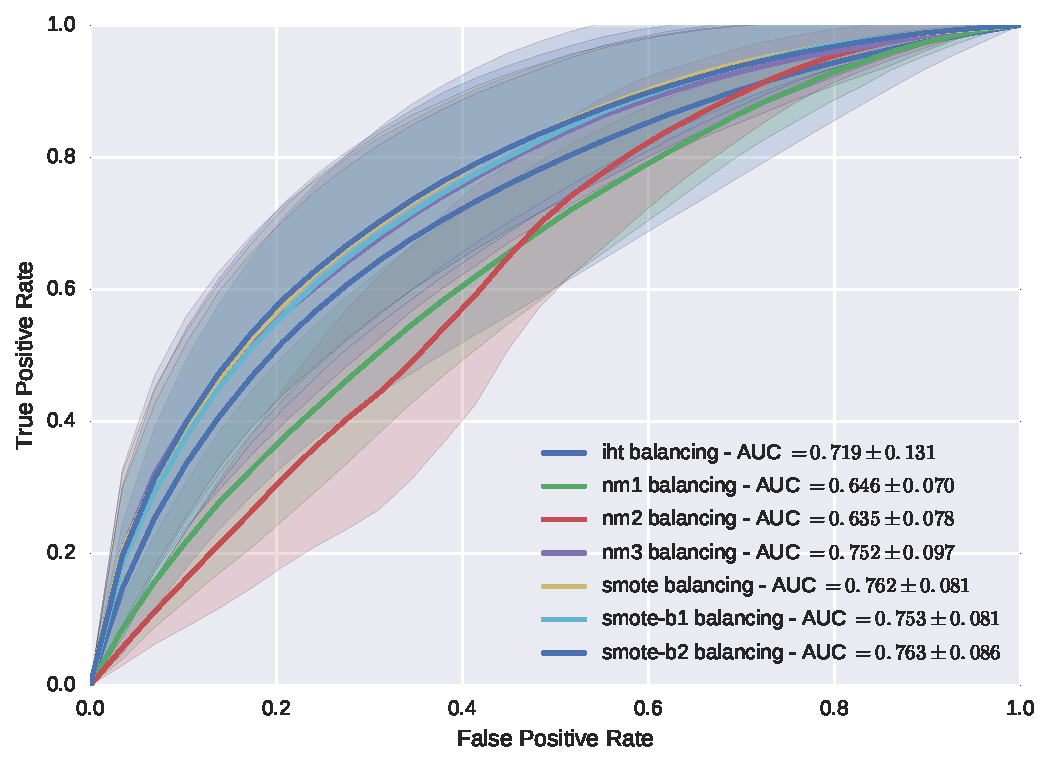
\includegraphics[width=.49\textwidth]{6_pipeline/figures/exp-3/t2w.pdf}}
  \hfill
  \subfigure[]{\label{fig:}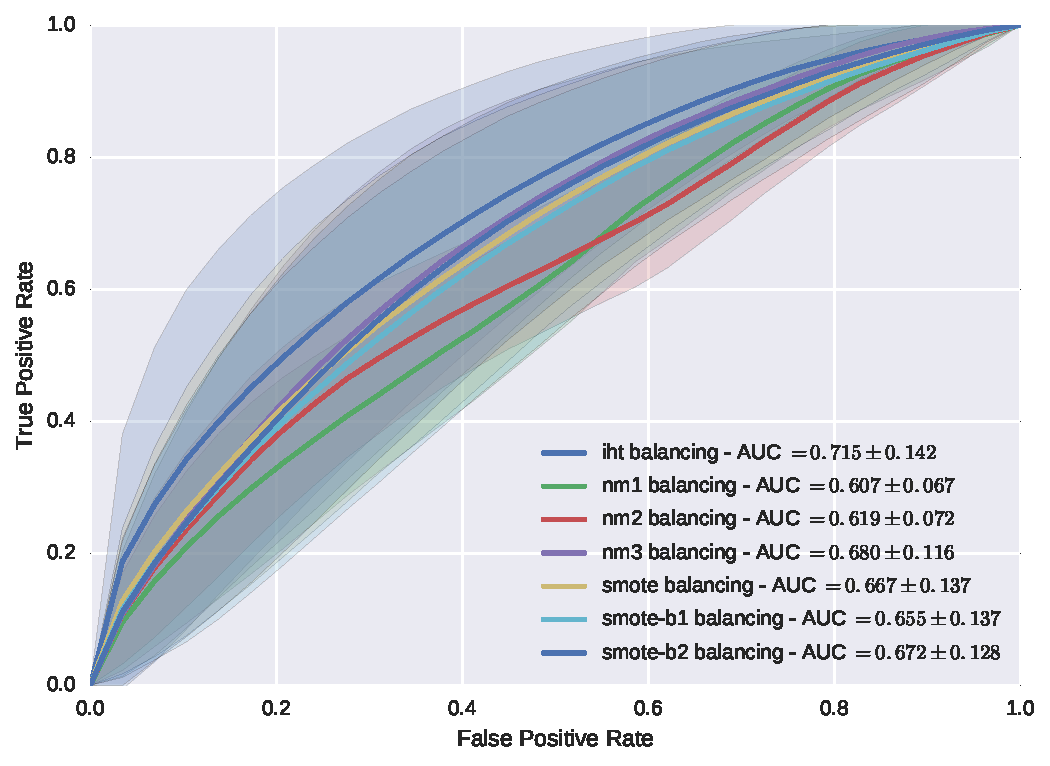
\includegraphics[width=.49\textwidth]{6_pipeline/figures/exp-3/adc.pdf}}
  \hspace*{\fill} \\
  \hspace*{\fill}
  \subfigure[]{\label{fig:}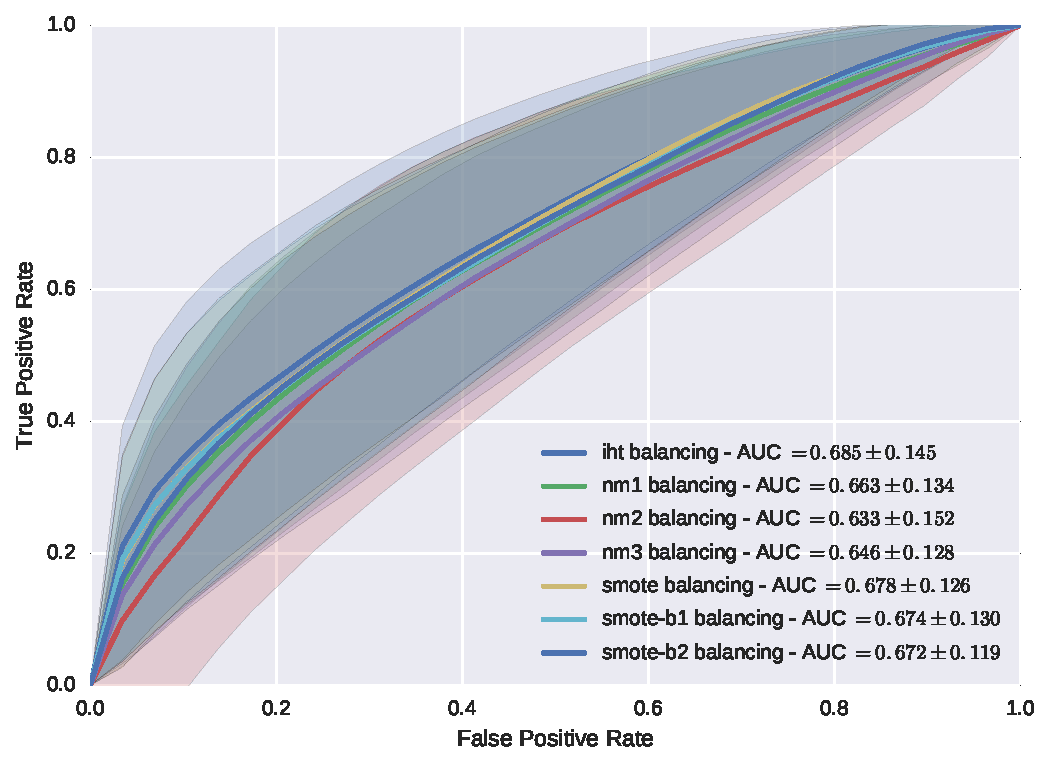
\includegraphics[width=.49\textwidth]{6_pipeline/figures/exp-3/dce.pdf}}
  \hfill
  \subfigure[]{\label{fig:}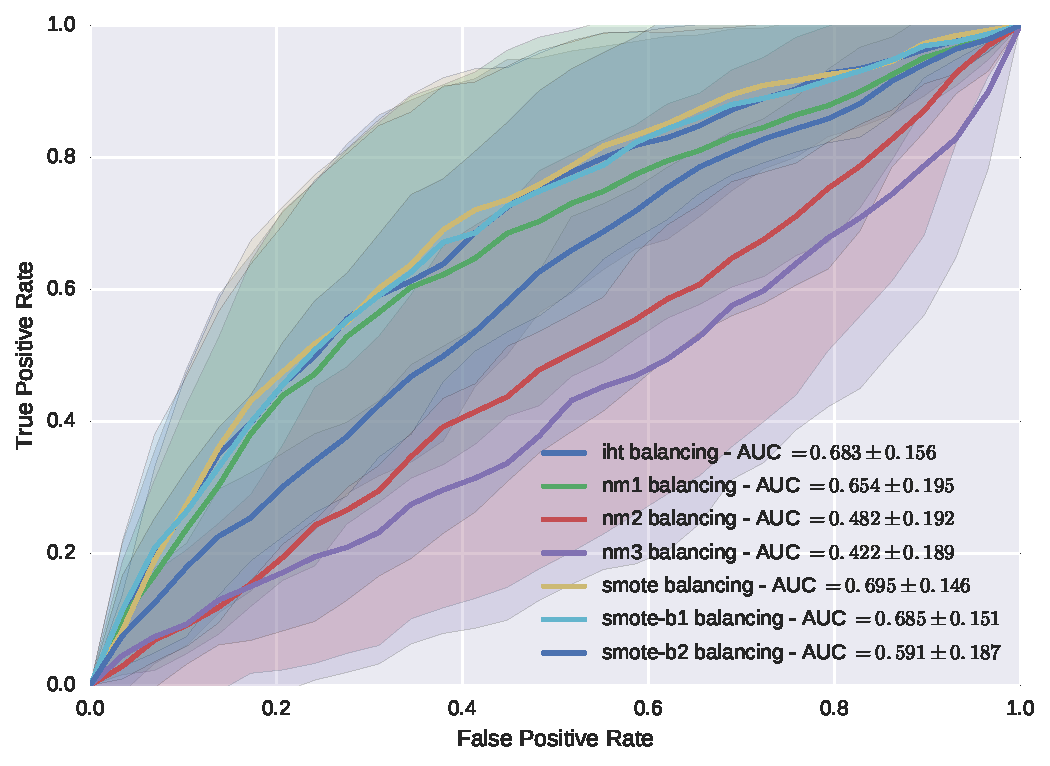
\includegraphics[width=.49\textwidth]{6_pipeline/figures/exp-3/mrsi.pdf}}
  \hspace*{\fill}
  \caption{Experiment 3:}
  \label{fig:}
\end{figure}

\begin{figure}
  \centering
  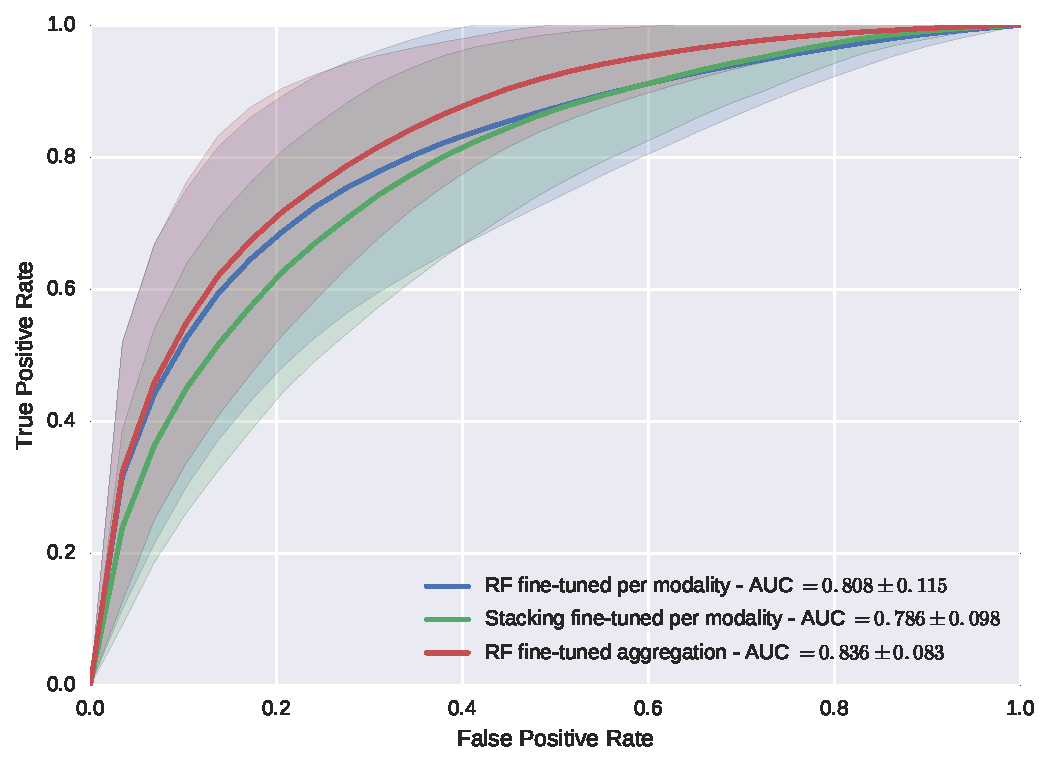
\includegraphics[width=0.7\linewidth]{6_pipeline/figures/exp-5/combine_all.pdf}
  \caption{Experiment 5:}
  \label{fig:}
\end{figure}
